\documentclass[12pt,a4paper]{article}

% Paquetes necesarios
\usepackage[utf8]{inputenc}  % Codificación UTF-8
\usepackage[spanish]{babel}  % Español
\usepackage{amsmath, amssymb, amsthm}  % Paquetes matemáticos
\usepackage{graphicx}  % Para incluir imágenes
\usepackage[margin=1in]{geometry}  % Márgenes
\usepackage{float}  % Para usar [H] en figuras
\usepackage{subcaption} % Para usar subfiguras
\usepackage{algorithm2e}  % Para escribir algoritmos

% Configuración del título
\title{\textbf{Trabajo Práctico 3}}
\author{\textbf{Alejo Ordoñez}\\ Universidad o Institución}
\date{\today}

\begin{document}

% Portada
\begin{titlepage}
    \centering
    \vspace*{5cm}

    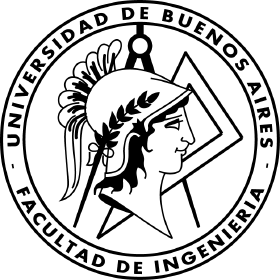
\includegraphics[width=0.4\textwidth]{logo-fiuba.png}\\[1cm]

    {\Huge \textbf{Trabajo Práctico 3}}\\[0.2cm]

    {\large \textbf{Aprendizaje Profundo}\\ Alejo Ordoñez}

    \vfill

    {\large 13 de diciembre de 2024}
\end{titlepage}

% Contenido principal
\section*{Resumen}
En este trabajo se presentan el algoritmo Simulated Annealing, para enseñar la función lógica XOR de dos entradas a un perceptrón multicapa, y el algoritmo de Kohonen, para entrenar una mapa auto-organizado con puntos con distribución uniforme en la circunferencia unitaria.

\newpage
\section{Simulated Annealing}
El simulated annealing es un algoritmo inspirado en el proceso de la metalurgia de enfriamiento de un metal, que se calienta y luego se enfría lentamente para reducir sus imperfecciones. La idea es simular estre proceso para minimizar una función de costo. Al principio se permite que la red explore el espacio de soluciones, aceptando soluciones peores con una probabilidad, con el objetivo de no quedar varados en un mínimo local malo. A medida que el tiempo avanza, la probabilidad de aceptar soluciones peores disminuye, permitiendo así que la red haga un fine-tunning de la solución.\\
Primero se elige una solución inicial $S$ y una función de costo $C$. Se parte de una temperatura inicial $\alpha$ y se itera perturbando la solución $S$ y aceptando o rechazando la solución perturbada $S'$ si $C(S') < C(S)$ o con una probabilidad que se computa como $\mathcal{U}(0, 1) < \exp[(C(S') - C(S))/\delta T]$, donde $\delta$ es un parámetro del algoritmo. En cada iteración se disminuye la temperatura multiplicándola por un factor $\epsilon$ hasta llegar a una temperatura final $\beta$.\\
Se entrenó un perceptrón multicapa para aprender la función lógica XOR de 2 entradas, con una capa oculta de 3 neuronas, usando simulated annealing. A continuación, se muestra la evolución del error en función de la temperatura.
\begin{figure}[H]
    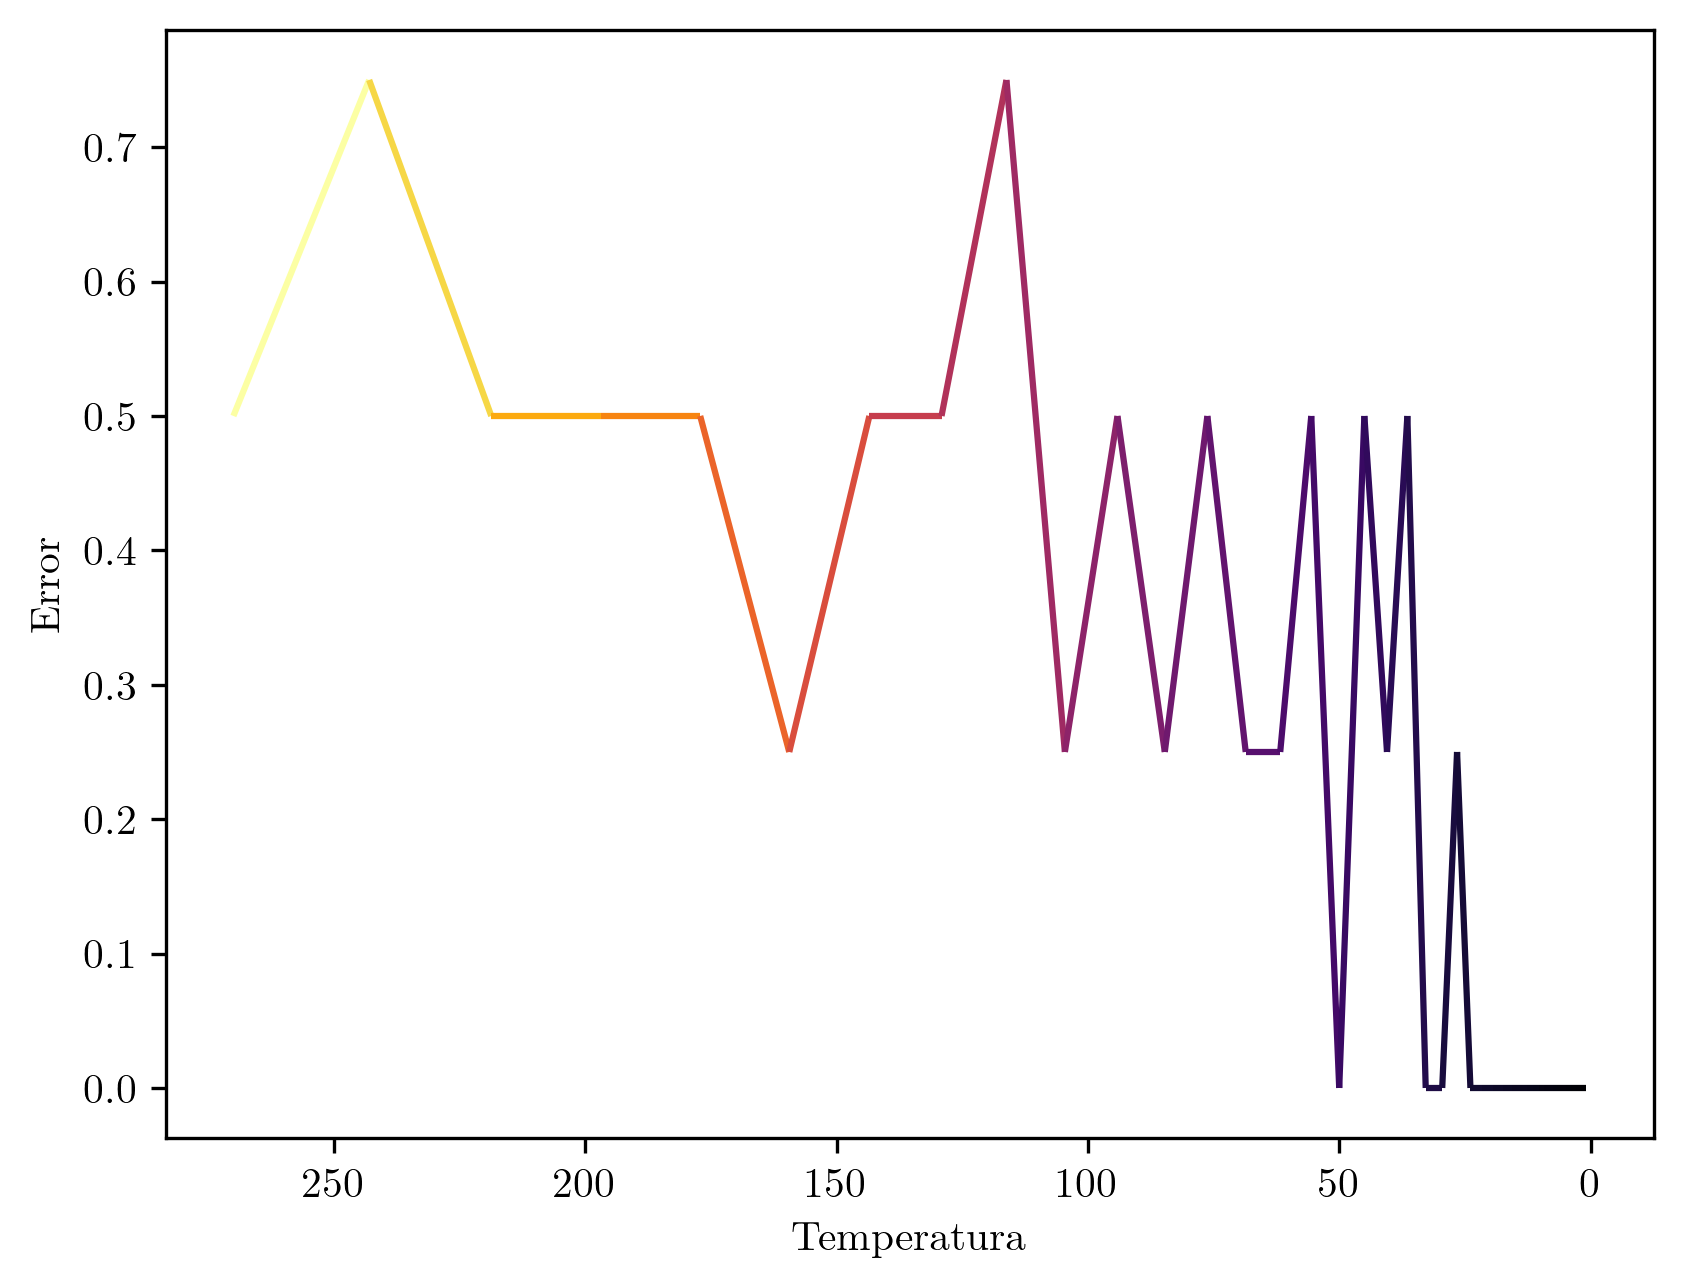
\includegraphics[width=0.6\textwidth]{img/simulated_annealing-error_xor.png}
    \centering
\end{figure}
\textit{Observar que el error no es necesariamente decreciente iteración a iteración}, ya que es posible que a lo largo del algoritmo se acepten soluciones peores, con menor probabilidad a medida que la temperatura disminuye. De igual manera, las mejores soluciones se van guardando y la elegida es la que tiene el menor costo.

\section{Red de Kohonen}
El algoritmo de Kohonen, se usa para entrenar mapas auto-organizados, para que aprendan a representar la distribución de los datos de entrada. La idea es unicar las neuronas de la red en una grilla que representa el espacio de salida. Cada neurona tiene asociado un peso, que vive en el espacio de las features del conjunto de datos. Se inicializan los pesos aleatoriamente, y se itera sobre los datos de entrada, actualizando los pesos de las neuronas cercanas a la neurona ganadora, que es la que tiene el peso más cercano al dato de entrada.\\
Hay $N$ valores continuamente valuados, $\xi_1$ a $\xi_N$, que definen un patrón $\boldsymbol\xi$. Las unidades de salida $O_i$ están dispuestas en una grilla (generalmente de una o dos dimensiones), y están todas conectadas con a las entradas vía los pesos $w_{ij}$. Se usa una regla de \textbf{competitiva}, para elegir la neurona ganadora $i^*$, que es la que tiene el peso más cercano al patrón de entrada $\boldsymbol\xi$:
$$
|\mathbf w_{i^*} - \boldsymbol\xi| \leq |\mathbf w_i - \boldsymbol\xi| \quad \text{(para todo } i \text{)}.
$$
La regla de aprendizaje de Kohonen es
\[
\Delta w_{ij} = \eta\Lambda (i, i^*) (\xi_j - w_{ij}) \label{eq:Kohonen}\tag{1}
\]
con $\eta = \eta_0 \exp(-t / tau)$, para todo $i$ y $j$. La \textbf{función de vecindad} $\Lambda(i, i^*)$ es 1 para $i = i^*$ y decrece con la distancia $|\mathbf r_i - \mathbf r_{i^*}|$ entre las neuronas $i$ y $i^*$ en la grilla. Por lo que los pesos de las neuronas cercanas a la ganadora, así como el de la ganadora misma, se actualizan considerablemente, mientras que las que están más lejos, para las cuáles $\Lambda(i, i^*)$ es pequeño, se actualizan en menor medida.\\
La regla (\ref{eq:Kohonen}) arrastra el vector de pesos $\mathbf w_{i^*}$ hacia el patrón de entrada $\boldsymbol\xi$. Pero también arrastra los pesos $\mathbf w_i$ con él. Es por esto que se puede pensar en una suerte de red elástica en el espacio de entrada que quiere acercarse tanto como sea posible a los patrones de entrada.\\
La función de vecindad que se eligió para el experimento es
$$
\Lambda(i, i^*) = \exp(-|\mathbf r_i - \mathbf r_{i^*}|^2/2\sigma^2)
$$
donde $\sigma$ está en función de la iteración $t$: $\sigma(t) = \sigma_0 \exp(-t / \tau)$, con $\sigma_0 = 1$ y $\tau$ la mitad de la cantidad de iteraciones del algoritmo.\\
A continuación se muestra la evolución de la topología de la grilla de pesos a lo largo de las iteraciones del aprendizaje de una distribución uniforme de puntos sobre la circunferencia unitaria $(r \cos \theta, r \sin \theta)$, con $r \sim \mathcal{U}(0.95; 1.05)$ y $\theta \sim \mathcal{U}(0, 2\pi)$.
\begin{figure}[H]
  \subcaptionbox*{}[.3\linewidth]{
    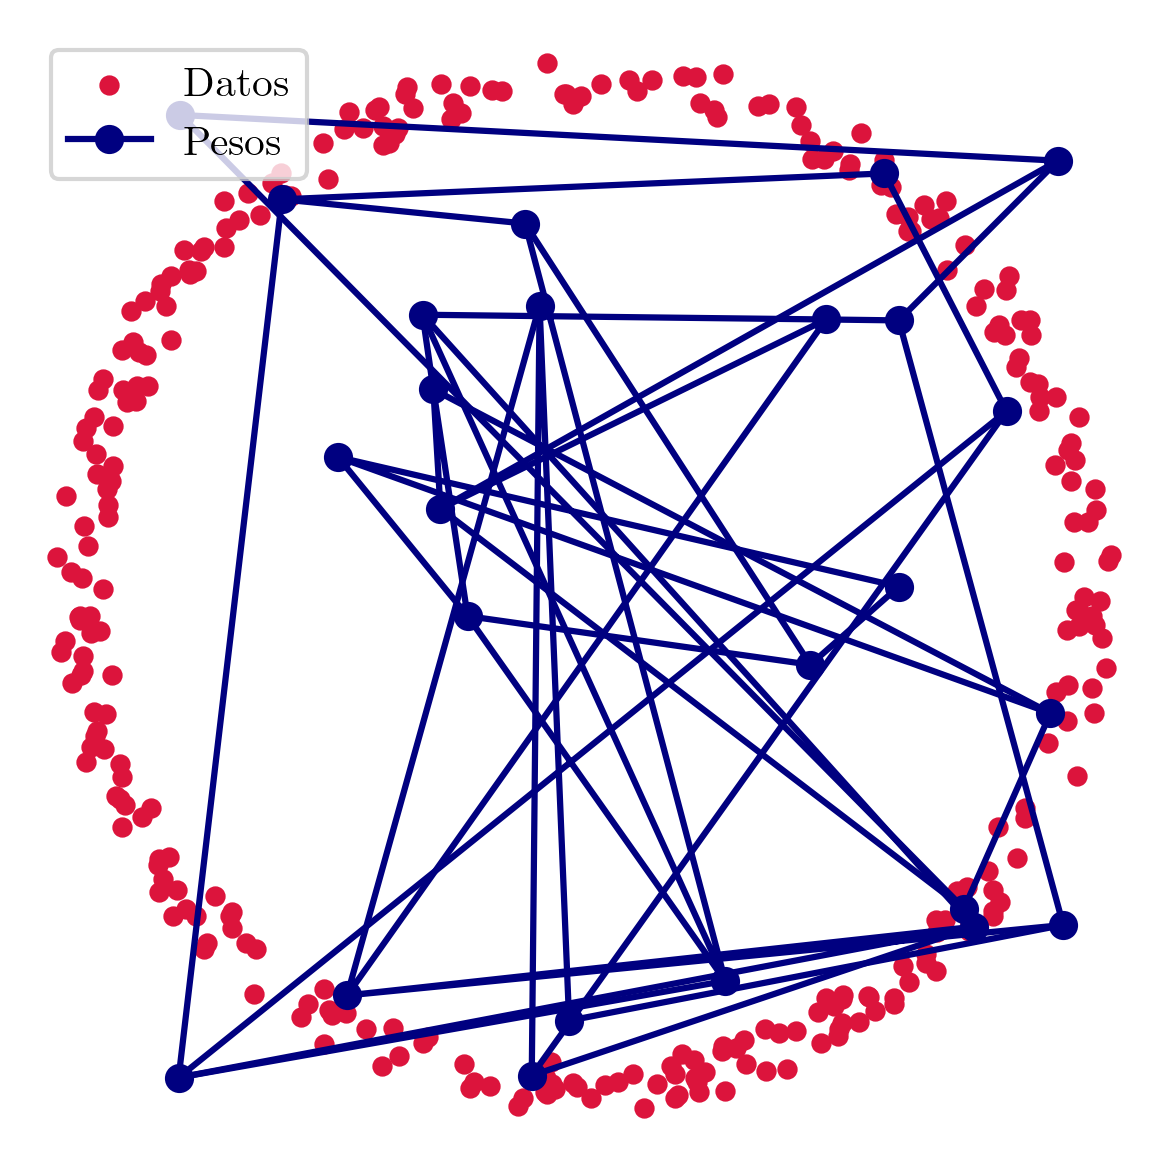
\includegraphics[width=\linewidth]{img/kohonen-topología_iteración0.png}
  }
  \subcaptionbox*{}[.3\linewidth]{
    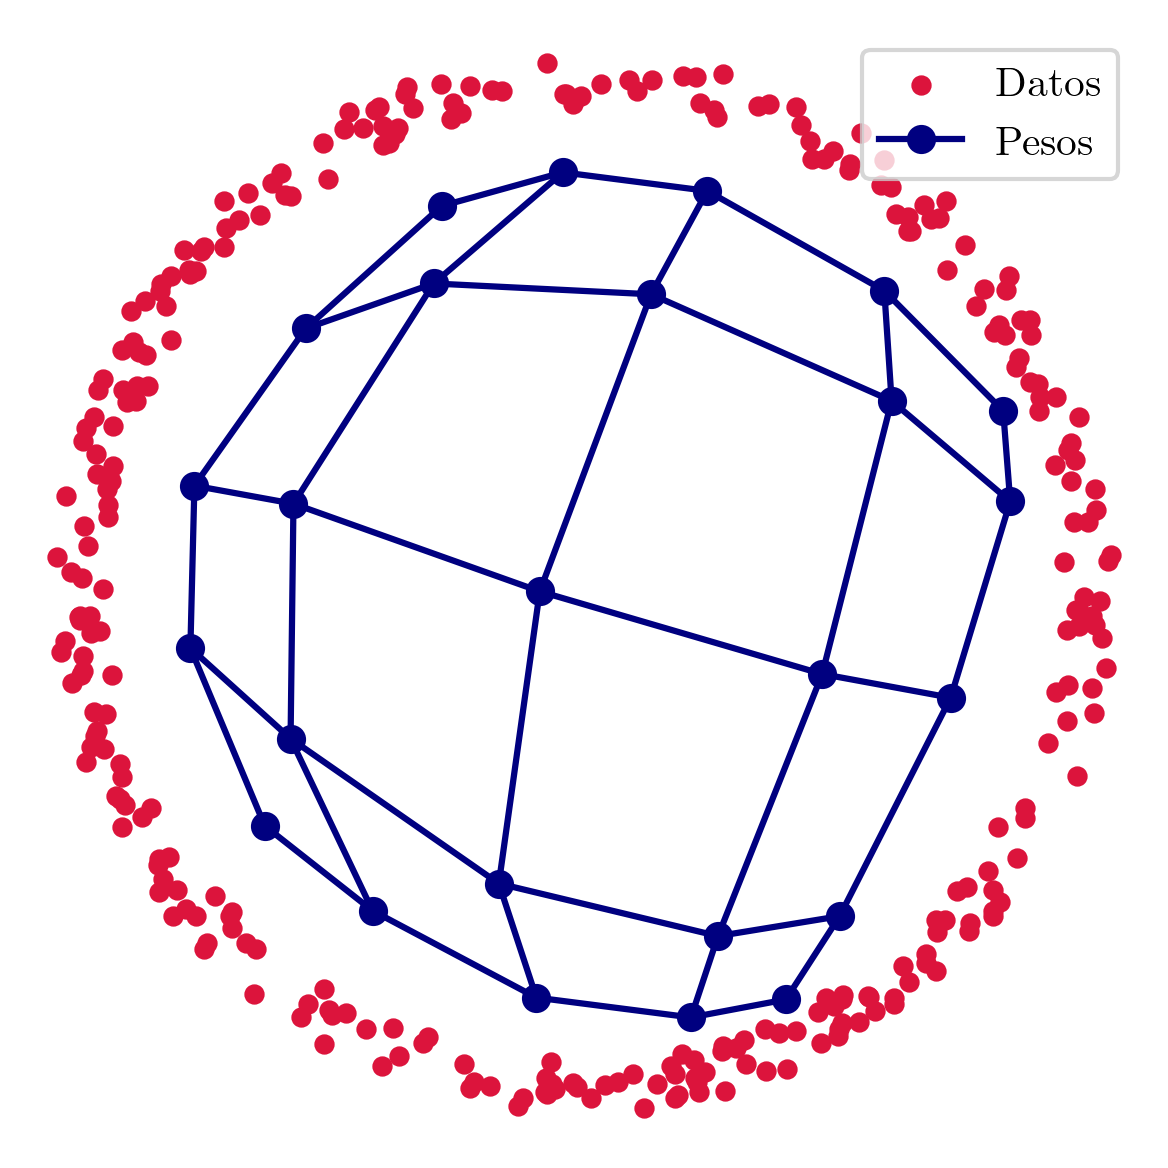
\includegraphics[width=\linewidth]{img/kohonen-topología_iteración10.png}
  }
  \subcaptionbox*{}[.3\linewidth]{
    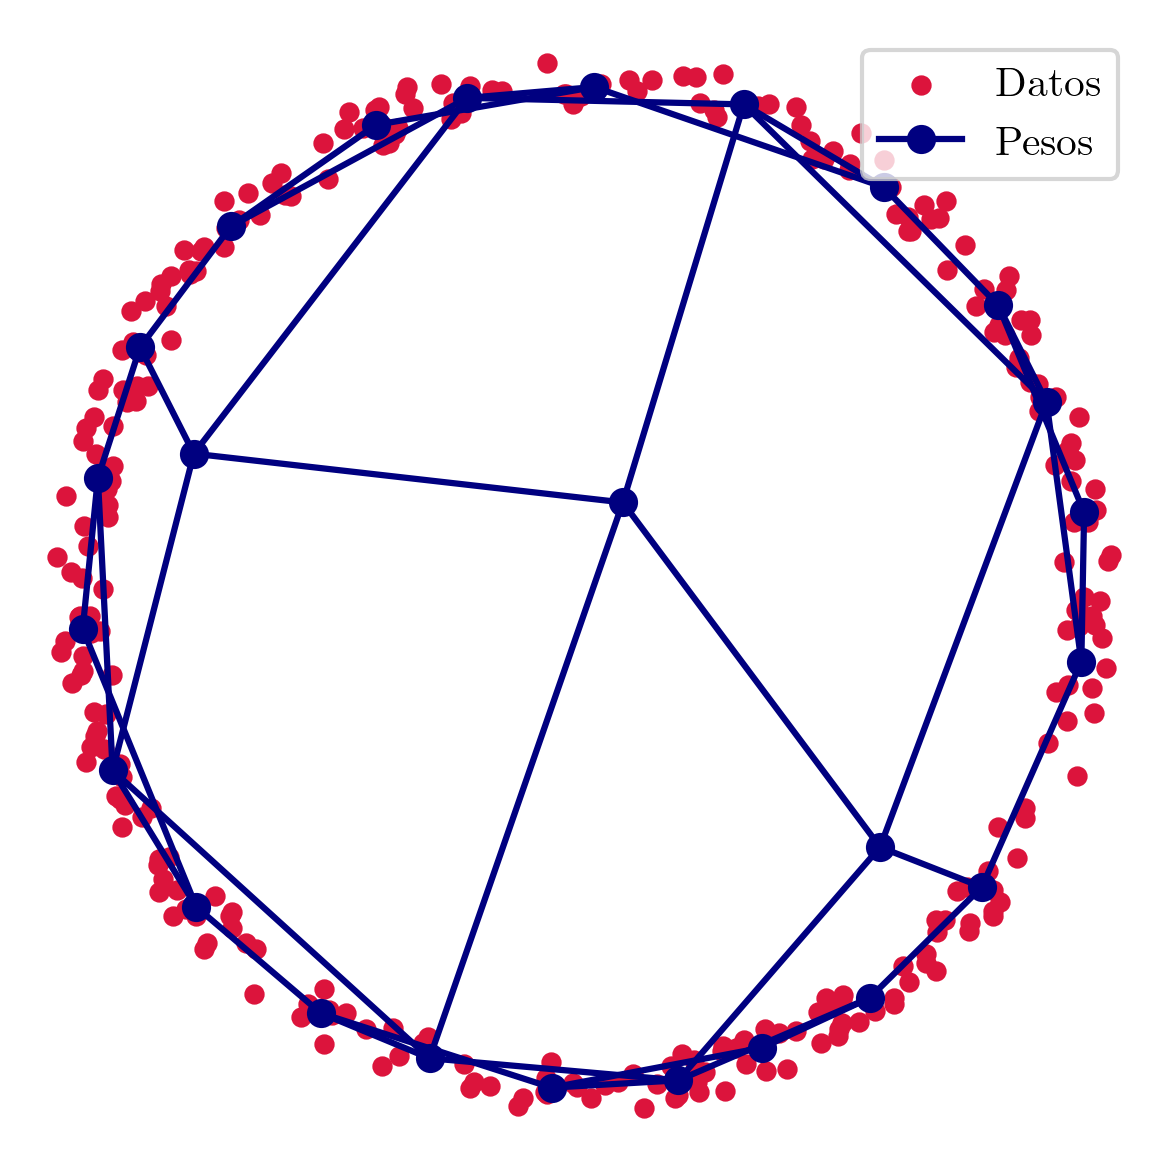
\includegraphics[width=\linewidth]{img/kohonen-topología_iteración100.png}
  }
  \centering
\end{figure}
De izquierda a derecha las imágenes muestran la topología de la red de pesos en la incialización, donde los pesos se vuelcan con una distribución uniforme en el espacio de entrada, en la décima iteración y en la centésima iteración. Se observa que la red de Kohonen logra representar la distribución de los datos de entrada, agrupando los pesos en las regiones donde hay más puntos.

% Bibliografía
\newpage
\begin{thebibliography}{9}
% John Hertz, Anders Krogh, Richard G. Palmer. Introduction to the Theory of Neural Computation
\bibitem{Introduction to the Theory of Neural Computation} John Hertz, Anders Krogh, Richard G. Palmer, \emph{Introduction to the Theory of Neural Computation}.
% Patrick Bangert. Optimizing Simulated Annealing
\bibitem{Optimizing Simulated Annealing} Patrick Bangert, \emph{Optimizing Simulated Annealing}.
% Teuvo Kohonen. The Self-Organizing Map
\bibitem{The Self-Organizing Map} Teuvo Kohonen, \emph{The Self-Organizing Map}.
\end{thebibliography}

\end{document}

